\section{Use Cases}

\subsection{Overview}

Before delving into the details of the specification it is useful to identify some of the key use cases for the technology. The use cases defined here are not an exhaustive list; however, they should help demonstrate how this specification is expected to be used and to help illustrate the benefits of a common information model.

\subsection{Device Maker}

The use case, shown in Figure \ref{fig:device_mfg_use_case}, centers on the manufacturer of a piece of equipment or device that needs to provide connectivity to other systems. In some cases, the device manufacturer will be targeting markets other than equipment (Machine Tool) and would benefit from a more generic specification like OPC UA. On the other hand, the standardized semantics of MTConnect are extremely important to standardized communications on the manufacturing shop floor. The MTConnect-OPC UA specification and the resulting standard information model allows the device manufacturers to standardize on OPC UA as the network interface while making their information accessible to software applications that includes the enhanced meaning and structure provided by applying the MTConnect semantics. Figure 1 shows several clients developed for different purposes that can access information produced by the device via OPC UA.

\begin{figure}[h]
  \centering
  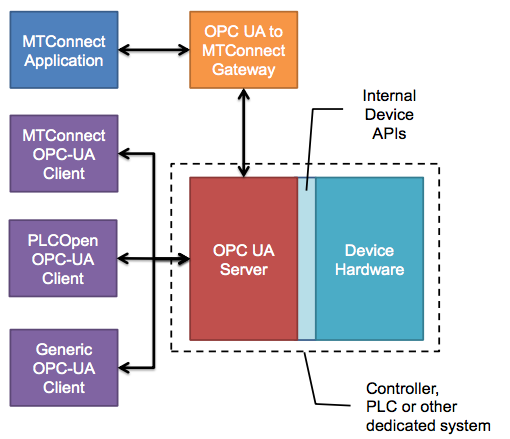
\includegraphics[width=0.75\textwidth]{diagrams/DeviceManufacturingUseCase.png}
  \caption{Device Manufacturer's Use Case}
  \label{fig:device_mfg_use_case}
\end{figure}

The device manufacture may also have a native MTConnect device and make use of an MTConnect to OPC UA gateway to provide the information to OPC UA aware clients (see Figure \ref{fig:device_mfg_native} and Figure \ref{fig:device_mfg_separate}). This standard allows for easy information flow between Client and Server that support either MTConnect or OPC UA.

The MTConnect or OPC UA interface may reside directly in the Machine, but it may also reside in some other device that communicates with the Machine. The actual location for the interface is up to the Machine vendor.

\textit{Should we add Minimum Level of OPC Functionality required to support this scenario}

\begin{figure}[h]
  \centering
  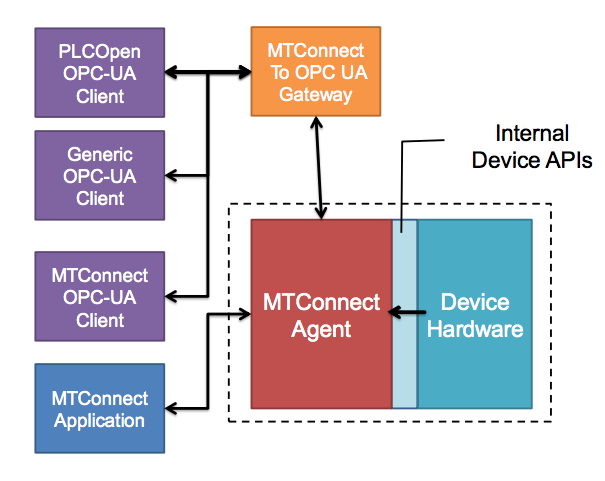
\includegraphics[width=0.75\textwidth]{diagrams/DeviceManufacturerNativeMTConnect.png}
  \caption{Device Manufacturer with Native MTConnect}
  \label{fig:device_mfg_native}
\end{figure}

\begin{figure}[h]
  \centering
  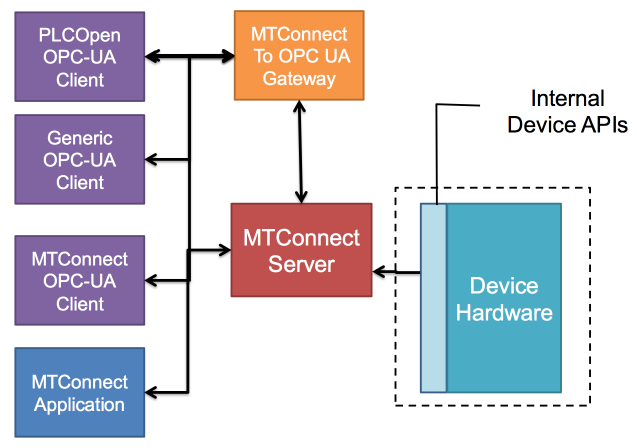
\includegraphics[width=0.75\textwidth]{diagrams/DeviceManufacturerSeparateAgent.png}
  \caption{Device Manufacturer with Separate MTConnect Agent}
  \label{fig:device_mfg_separate}
\end{figure}

\FloatBarrier

\subsubsection{Independent Software Vendor}

The use case shown in Figure \ref{fig:isv_use_case} centers on an Independent Software Vendor (ISV) that wishes to sell products to users of equipment such as Machine Tools. An ISV will typically want to provide gateways that convert information between MTConnect and OPC UA as well as adding numerous features that add value to the semantics defined in the MTConnect standards. The MTConnect-OPC UA specification allows the ISV to extend the MTConnect-OPC UA information model with application specific constructs which can be easily accessed via any standard OPC UA client product. These added features will exist in parallel to the standard MTConnect interfaces. Figure \ref{fig:isv_use_case} shows an ISV product that consumes data from MTConnect and OPC UA enabled devices and then makes it available via MTConnect and OPC UA.

\begin{figure}[h]
  \centering
  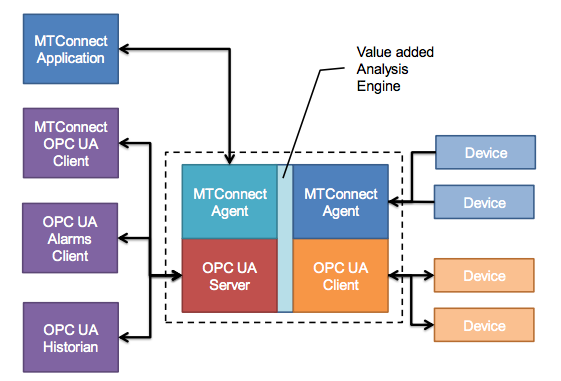
\includegraphics[width=0.75\textwidth]{diagrams/ISVUseCase.png}
  \caption{The Independent Software Vendor (ISV) Use Case}
  \label{fig:isv_use_case}
\end{figure}

\subsection{End-User Engineer}

This use case shown in Figure \ref{fig:end_user_use_case} centers on an Engineer or Systems Integrator responsible for setting up and configuring an MTConnect enabled system for a user of Machine Tools. The Engineer is typically familiar with the MTConnect specification but wishes to configure generic OPC UA client applications. The MTConnect-OPC UA specification allows the Engineer to understand how MTConnect concepts are represented in OPC UA and determine what they need to do to configure their OPC UA Applications. Without this specification, an Engineer interested in OPC based data would have had to rely on vendor documentation and a laborious process of manually mapping tags to MTConnect concepts. This specification eliminates the need for that by providing a standard mapping. Figure \ref{fig:end_user_use_case} shows how the common Information Model defined by this specification gives the End User Engineer choices when it comes to accessing device data.\

\begin{figure}[h]
  \centering
  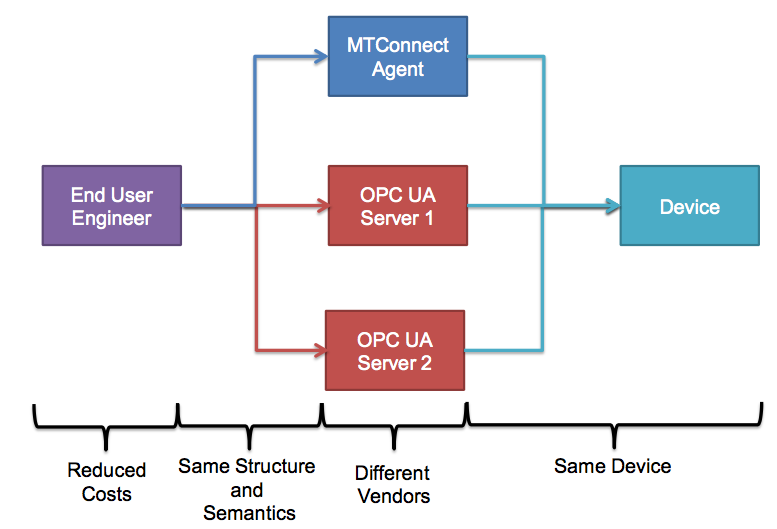
\includegraphics[width=0.75\textwidth]{diagrams/EndUserUseCase.png}
  \caption{End User Engineering Use Case}
  \label{fig:end_user_use_case}
\end{figure}
